\section{AVHRR infrared channel SRF comparison}
%==============================================
\label{app:n16}
In the processing of the official SRF data from the 
\href{http://www.star.nesdis.noaa.gov/smcd/spb/fwu/solar_cal/spec_resp_func}{NESDIS/STAR website}
an initial procedure was applied to eliminate all relative responses
less than 1.00E-4. For NOAA-16 channel 3B relative responses at the periphery
of the main response features are unchanging with respect to frequency, but
exceed 1.00E-4 as shown in the following plots. 
As a result of this finding visual inspection was used to eliminate extraneous data
from the official SRF datasets.
Data is eliminated if either of the following two criteria are met:
1) The data appears to be unchanging with frequency. 2) The position of
a zero crossing in relative response is closer to the main response
features than the data sample being considered. Table \ref{tab:N16_teff}
demonstrates that the radiometric impact of eliminating the data is significant.
The plots in figures \ref{fig:nocutoff_complete}, \ref{fig:cutoff_complete} 
and \ref{fig:cutoff_inspection} show the cutoff frequency points that were assigned based 
on visual inspection. 

\begin{figure}[htp]
  \centering
  \includegraphics[scale=1]{graphics/nominal/nocutoff_complete.eps}
  \caption{Plot of NOAA-16 channel 3B SRF's with cutoff from visual inspection depicted
           by red dashed line.}
  \label{fig:nocutoff_complete}
\end{figure}

\begin{figure}[htp]
  \centering
  \includegraphics[scale=1]{graphics/nominal/cutoff_complete.eps}
  \caption{Plot of NOAA-16 channel 3B SRF's with cutoff from visual inspection depicted
           by red dashed line. Extraneous data has been removed from this plot.}
  \label{fig:cutoff_complete}
\end{figure}

\begin{figure}[htp]
  \centering
  \includegraphics[scale=1]{graphics/zoom/cutoff_inspection.eps}
  \caption{These plots provide a zoom in look at the cutoff points. The
   plots demonstrate the selection of cutoff points by visual inspection.}
  \label{fig:cutoff_inspection}
\end{figure}
\newpage

\begin{table}[ht]
  \centering
  \begin{tabular}{| l | r |}
    \hline
    \hline
    No Cutoff & 286.25 \\
    \hline
    Cutoff & 286.12 \\
    \hline
    Current & 286.09 \\
    \hline
  \end{tabular}
  \caption{NOAA-16 effective temperatures for a blackbody temperature of 285K.}
  \label{tab:N16_teff}
\end{table}
 
